%-------------------------
% Rover Resume - Fancy Template
% Link: https://github.com/subidit/rover-resume
%------------------------

\documentclass[11pt]{article}

\usepackage[T1]{fontenc}
\usepackage{inter} % https://tug.org/FontCatalogue/
\renewcommand*\familydefault{\sfdefault}
\usepackage{graphicx}

\usepackage{geometry}
\geometry{
a4paper,
top=1.8cm,
bottom=1in,
left=2.5cm,
right=2.5cm
}

\setcounter{secnumdepth}{0} % remove section numbering
\pdfgentounicode=1 % make ATS friendly

\usepackage{enumitem}
\setlist[itemize]{
    noitemsep,
    left=0pt..1.5em
}
\setlist[description]{itemsep=0pt}
\setlist[enumerate]{align=left}

\usepackage[dvipsnames]{xcolor}
% \usepackage[dvipsnames, svgnames, x11names]{xcolor} 
% \usepackage[dvipsnames]{xcolor} % xcolor.pdf Sec.4 Colors by Name
\colorlet{icnclr}{gray}
% \colorlet [⟨type⟩]{⟨name⟩}[⟨num model⟩]{⟨color ⟩}
% \definecolor[⟨type⟩]{⟨name⟩}{⟨model-list⟩}{⟨spec-list⟩}


\usepackage{titlesec}
% \titlespacing{command}{left spacing}{before spacing}{after spacing}[right]
% \titlespacing{\section}{0pt}{*3}{*1}
\titlespacing{\subsection}{0pt}{*0}{*0}
\titlespacing{\subsubsection}{0pt}{*0}{*0}
% \titleformat{<command>}[<shape>]{<format>}{<label>}{<sec>}{<before-code>}[<after-code>]  
\titleformat{\section}{\color{Sepia}\large\fontseries{black}\selectfont\uppercase}{}{}{\ruleafter}[\global\RemVStrue]
\titleformat{\subsection}{\large\fontseries{semibold}\selectfont}{}{}{\rvs}
\titleformat{\subsubsection}{\large\fontseries{medium}\selectfont}{}{}{}

\usepackage{xhfill} 
\newcommand\ruleafter[1]{#1~\xrfill[.5ex]{1pt}[gray]} % add rule after title in .5 x-height 

\newif\ifRemVS % remove vspace between \section & \subsection
\newcommand{\rvs}{
    \ifRemVS
        \vspace{-1.5ex}
    \fi
    \global\RemVSfalse
}


\usepackage{fontawesome5}

\usepackage[bookmarks=false]{hyperref} % [imp!]
\hypersetup{ % https://en.wikibooks.org/wiki/LaTeX/Hyperlinks
    colorlinks=true,
    urlcolor=Sepia,
    pdftitle={My Resume},
}

\usepackage[page]{totalcount}
\usepackage{fancyhdr}
\pagestyle{fancy}
\renewcommand{\headrulewidth}{0pt}	
\fancyhf{}							
\cfoot{\color{darkgray} Alessio Rovere CV (ENG) -- Page \thepage{} of \totalpages}


\usepackage[backend=biber,style=apa,sorting=ydnt,uniquename=false,isbn=false,maxbibnames=99,url=false,giveninits=true,eprint=false]{biblatex}
\AtEveryBibitem{\clearfield{note}}
\addbibresource{sample.bib}


\begin{document}

%== HEADER ==%
\begin{center}
    {\fontsize{36}{36}\selectfont\interthin Alessio \interheavy Rovere} \\ \bigskip
    {\fontsize{14}{14}\selectfont\interthin Curriculum Vitae - English version}\\ \bigskip
    {\color{icnclr}\faEnvelope[regular]} \href{mailto:alessio.rovere@unive.it}{alessio.rovere@unive.it}
\end{center}

\section{Education}
{\normalfont My academic journey took place at the University of Genoa, Italy, renowned for its excellence in environmental and geosciences. During my Ph.D., I spent several visiting periods abroad as a visiting Ph.D. student.} \\

%==============
\bigskip
\subsection{Università degli Studi di Genova $|$ {\normalfont\textit{Ph.D. in Marine Sciences}} \hfill 06/2011}
{\footnotesize My PhD holds the "European PhD label," which mandates rigorous standards. This includes thesis review by two professors from different European countries, the participation of at least one jury member from a different European country, and conducting the defense in an official EU language distinct from the thesis country. Additionally, the research leading to the thesis involved a minimum six-month period in another European country. Main advisor: Prof. Marco Firpo.}\\
{\footnotesize 
\textbf{Visiting periods during the Ph.D.}
\begin{description}
  \item [2010] University of Western Australia, AU (1 month).
  \item [2010] Brunel University, UK (4 months).
  \item [2010] University of the Aegean, GR (17 days).
  \item [2009] University of the Aegean, GR (1 month).
\end{description}}
\bigskip

\subsection{Università degli Studi di Genova $|$ {\normalfont\textit{MSc in Marine Environmental Sciences}} \hfill 07/2006}
{\footnotesize Two-years master course in marine environmental sciences. During these two years, I was awarded an ERASMUS Scholarship. Final mark: 110/110. Main advisor: Prof. Marco Firpo.}\\
{\footnotesize 
\textbf{ERASMUS Scholarship}
\begin{description}
  \item [2004] Universidad de Las Palmas de Gran Canaria, ES (3 months, 18 days)
\end{description}
\bigskip}

\subsection{Università degli Studi di Genova $|$ {\normalfont\textit{BSc in Environmental Sciences}} \hfill 02/2004}
{\footnotesize Three-years bachelor course in environmental sciences. Final mark: 110/110. Main advisor: Prof. Carlo Nike Bianchi.}

\section{Academic work experience}
{\normalfont My post-Ph.D. academic journey has predominantly unfolded abroad. I spent 2 years in the USA (Columbia University, ranked 17th in the World University Rankings 2024 by THE) and 8 years in Germany (Universität Bremen, a German "University of Excellence") before returning to Italy in 2021. I have been leading my own research group independendly since 03/2014 (2 years and 9 months after I obtained my Ph.D.)}\\
%============
\bigskip
\subsection{Università Ca' Foscari Venezia  $|$ {\normalfont\textit{Associate Professor}} \hfill 11/2021 - Present}
{\footnotesize The Associate Professor role includes teaching, research and faculty administration duties. I manage my own research group, which currently counts four postdoctoral researchers. I was hired at Ca' Foscari throuhg a direct appointment following the positive evaluation of the italian Ministry for University and Research (prot. n. 11888 del 4.09.2021, following art. 1 comma 9 of the Law n. 230/2005}
\bigskip

\subsection{Universität Bremen  $|$ {\normalfont\textit{Professor}} \hfill 04/2020 - 10/2021}
{\footnotesize In addition to my position as "Research Scientist," I have been conferred the title of "Professor" in accordance with Article 17 of the Higher Education Act of the State of Bremen.}
\bigskip

\subsection{Universität Bremen  $|$ {\normalfont\textit{Research scientist}} \hfill 03/2019 - 10/2021}
{\footnotesize As a tenured independent research scientist at MARUM (Center for Marine Environmental Sciences), affiliated with the University of Bremen, I spearheaded my research group, "Sea Level and Coastal Changes." My responsibilities encompassed leading research initiatives and fulfilling teaching obligations at the University of Bremen, alongside my primary focus on research endeavors.}
\bigskip

\subsection{Universität Bremen and Leibniz ZMT $|$ {\normalfont\textit{Young group leader}} \hfill 03/2014 - 02/2019}
{\footnotesize As a tenure-track young investigator group leader at MARUM (Center for Marine Environmental Sciences) and the Leibniz Centre for Tropical Marine Research (ZMT), I initiated and led the research group, "Sea Level and Coastal Changes." My role involved establishing myself as a leader in the field, driving research initiatives and applying for funding. I also contributed to teaching activities at the University of Bremen.}
\bigskip

\subsection{Columbia University $|$ {\normalfont\textit{Postdoctoral researcher}} \hfill 02/2012 - 02/2014}
{\footnotesize As a postdoctoral research scientist at Lamont Doherty Earth Observatory (Columbia University) I performed research within the NSF-funded project PLIOMAX. Advisor: Prof. Maureen E. Raymo.}
\bigskip

\section{Technological transfer}
{\normalfont While pursuing my Ph.D. at the University of Genoa, I co-founded SeaMap srl, an environmental consulting company, in collaboration with six other partners. The company received startup funds from a consortium initiated by the University of Genoa (UNITI) and was later recognized as a spinoff company of the same university. As director from 2010 to 2016, I oversaw its operations until its closure in 2017. In 2011, SeaMap received the "Italia degli Innovatori" prize from the "Agenzia per la diffusione delle tecnologie per l’innovazione - Presidenza del Consiglio dei Ministri."}\\
%============
\bigskip
\subsection{SeaMap srl  $|$ {\normalfont\textit{Director}} \hfill 10/2010 - 12/2016}
{\footnotesize As Director (Amministratore Unico), I led both the technical and administrative facets of commercial projects, overseeing research and development activities. I was responsible for managing the utilization of startup funds (32.000 euros) and effectively handled approximately 120.000 euros worth of commercial projects (excluding VAT).}
\bigskip

\section{Other research or teaching positions}
{\normalfont In addition to my academic work positions, I held several appointments, either as adjucnt faculty or visiting researcher.}\\
%============
\bigskip
\subsection{Universität Bremen  $|$ {\normalfont\textit{Honorary Professor}} \hfill 03/2024 - Present}
{\footnotesize The University of Bremen's committee has conferred upon me the title of Honorary Professor. This appointment, renewable every five years, entails active engagement in teaching and collaborative research activities. Additionally, it grants me the official authority to supervise Ph.D. students at the University of Bremen.}
\bigskip

\subsection{MARUM - Universität Bremen  $|$ {\normalfont\textit{External member}} \hfill 10/2021 - Present}
{\footnotesize A MARUM external member is expected to actively engage in research activities within the designated cluster, dedicating time to project meetings, participating in thesis committees, and similar commitments. Furthermore, acknowledgment of dual affiliation in publications is encouraged when appropriate.}
\bigskip

\subsection{LDEO - Columbia University  $|$ {\normalfont\textit{Adjucnt Research Scientist}} \hfill 04/2014 - 08/2021}
{\footnotesize As an adjunct at LDEO, my role involved engaging in research activities at the Observatory while concurrently maintaining my primary affiliation with another institution.}
\bigskip


\section{University service}
%===============
{\normalfont As an Associate Professor at Ca'Foscari University, I have undertaken various responsibilities in overseeing and managing both teaching and research activities.}\\
%============
\bigskip
\subsection{Università Ca' Foscari Venezia  $|$ {\normalfont\textit{Teaching coordinator}} \hfill 04/2024 - Present}
{\footnotesize As the Teaching Coordinator of the courses in Environmental Sciences (BSc and MSc), my responsibility is to oversee the activities of the Study Programme, encompassing both its planning and implementation aspects, and ensuring continuous review of the pathways for improvement. I actively pursue and promote the Quality Assurance process of the Study Programme, striving to make it effective and aligned with the strategic objectives of the University and Department. I ensure conformity with the University's Quality Assurance system and the guidelines of the National Agency for the Evaluation of the University and Research Systems (ANVUR). Nominated by Ca' Foscari DAIS Department Council on 26.03.2024.}
\bigskip

\subsection{Università Ca' Foscari Venezia  $|$ {\normalfont\textit{ERASMUS commission}} \hfill 12/2022 - Present}
{\footnotesize As a Member of the "Erasmus Commission for Environmental Sciences," I assist in overseeing ERASMUS scholarship requests and contribute to the internationalization of our student body. Nominated by Ca' Foscari DAIS Department Council on 13.12.2022.}
\bigskip

\subsection{Università Ca' Foscari Venezia  $|$ {\normalfont\textit{ERC Board member}} \hfill 09/2022 - Present}
{\footnotesize As a member of the "Ca' Foscari ERC Board" (appointed by Ca' Foscari Rector’s Decree 815/2022), I evaluate applications and act as a liaison between my Department and Principal Investigators of ERC grants who initially selected a different Italian or foreign institution as their Host Institution but intend to transfer to Ca' Foscari. I actively seek out talented researchers and initiate contact with them.}
\bigskip

\subsection{Università Ca' Foscari Venezia  $|$ {\normalfont\textit{ESA Lab Steering Committee}} \hfill 2022 - Present}
{\footnotesize I am member of the "ESA Lab@CaFoscari" Steering Committee (Ca' Foscari and European Space Agency), which promotes, coordinates, and supports research activities, scientific collaborations, teaching initiatives, and scientific events related to space data and research.}
\bigskip

\section{Other Institutional service}
%===============
%============
\bigskip

\subsection{Università Ca' Foscari Venezia  $|$ {\normalfont\textit{Ph.D. Program Board}} \hfill 05/2023 - Present}
{\footnotesize I am a member of the Ph.D. Program Board (Collegio di dottorato) in the "Doctoral of National Interest in Polar Sciences" at Ca' Foscari University of Venice.}
\bigskip

\subsection{Università Ca' Foscari Venezia  $|$ {\normalfont\textit{Ph.D. Program Board}} \hfill 05/2022 - Present}
{\footnotesize I am a member of the Ph.D. Program Board (Collegio di dottorato) in "Polar Sciences" at Ca' Foscari University of Venice.}
\bigskip

\subsection{MPA "Cinque Terre"  $|$ {\normalfont\textit{Scientific Committee member}} \hfill 06/2021 - Present}
{\footnotesize As a member of the Scientific Committee of the Marine Protected Area (MPA) "Cinque Terre," I contribute to overseeing scientific activities within the MPA and provide guidance on technical and scientific matters pertaining to MPA management.}
\bigskip

\newpage
\section{Service for international research organisations}
%===============
{\normalfont I am an active member of the international scientific community working on paleo sea-level changes and, more broadly, coastal processes.}\\
%============
\bigskip
\subsection{INQUA  $|$ {\normalfont\textit{CMP Commission President}} \hfill 2023 - Present}
{\footnotesize As President of the Coastal and Marine Processes Commission of the International Union for Quaternary Sciences, I play a key role in guiding strategic decisions and oversee funding applications for conferences and workshops.}
\bigskip

\subsection{SCAR-INSTANT  $|$ {\normalfont\textit{Steering Committee}} \hfill 2022 - Present}
{\footnotesize As a member of the Steering Committee of the Instabilities and Thresholds in Antarctica (INSTANT) project under the Scientific Committee on Antarctic Research (SCAR), I help steer decisions on the project's scientific directions and play an advisory role.}
\bigskip

\subsection{PALSEA  $|$ {\normalfont\textit{Co-Leader}} \hfill 2018 - 2023}
{\footnotesize I served as the co-leader (with other three scientists) of the PALSEA (PALeo constraints on SEA level rise) project, funded by INQUA and PAGES to support yearly workshops and training schools. In this role, I directed strategic decisions on the project's scientific focus, promoted activities to expand its scope, and decided on travel funding applications from early career researchers.}
\bigskip

\subsection{MEDFLOOD  $|$ {\normalfont\textit{Co-Leader}} \hfill 2012 - 2016}
{\footnotesize I served as the co-leader (with other three scientists) of the MEDFLOOD project, funded by INQUA to support yearly workshops and training schools on Mediterranean sea-level science. In this role, I directed strategic decisions on the project's scientific focus, promoted activities to expand its scope, and decided on travel funding applications from early career researchers.}
\bigskip

\section{Scientific Committees of conferences}
%===============
{\normalfont Throughout my career, I have actively organized meetings and proposed sessions for international conferences. Below is a list of conferences and workshops where I served on the organizing committee or took on the role of session organizer, convener, or chair.}\\

\bigskip
{\normalfont 
\subsection{Member of scientific and organisation committees}
{\footnotesize
\begin{description}
  \item [2022] PALSEA annual meeting, Singapore.
  \item [2021] Webinar series by PALSEA, WCRP (sea level), IAG, and SERCE.
  \item [2020] "PALSEA Express" online workshop.
  \item [2019] CoChE Summer school. Coastal Changes and Evolution. Oristano (IT).
  \item [2019] PALSEA workshop "Using ecological and chronological data to improve proxy-based paleo sea level reconstructions", Dublin (IE).
  \item [2017] PALSEA-QUIGS meeting on “Climate, ice sheets and sea level during past interglacial periods”. Galloway, New Jersey (USA)
  \item [2012] Annual MEDFLOOD workshop, Rome (IT).
  \item [2014] Annual MEDFLOOD workshop, Haifa (IL).
  \item [2016] Annual MEDFLOOD workshop, Bremen (DE)
  \item [2013] Organizer of the bi-weekly seminar at Lamont Doherty Earth Observatory, Biology and Paleo Environment Division
  \item \end{description}}}

{\normalfont 
\subsection{Session organiser, convener or chair}
{\footnotesize
\begin{description}
  \item [2023] Rome INQUA conference. Session 89: "Cenozoic sea-level indicators and ice sheet constraints to global sea-level change".
  \item [2022] PAGES Open Science Meeting. Session: "Last Interglacial".
  \item [2019] American Geophysical Union 2019. Session PP23A: "Centennial Session: One Hundred Years of Ice Sheet and Sea Level Science".
  \item [2017] GeoBremen conference. Session: "Coastal depositional environments \& processes"
  \item [2015] American Geophysical Union 2015. Session PP11E: "Sea Levels and Ice Sheets during Past Warm Periods: Looking to the Past to Understand the Future".
  \item \end{description}}}

\section{Editorial and Reviewer roles}
{\normalfont Throughout my career, I have served in various editorial and reviewer roles for international journals.}\\

%===============
\bigskip

\subsection{Earth System Science Data  $|$ {\normalfont\textit{Editor}} \hfill 2022 - Present}
{\footnotesize I am an editor of Earth System Science Data, an open-access journal published by Copernicus. The journal has a 2022 impact factor of 11.4. For this journal, I edited 15 manuscripts.}
\bigskip

\subsection{Climate of the Past  $|$ {\normalfont\textit{Editor}} \hfill 2022 - Present}
{\footnotesize I am an editor of Climate of the Past, an open-access journal published by Copernicus. The journal has a 2022 impact factor of 4.3. For this journal, I edited 21 manuscripts.}
\bigskip

\subsection{UAVs in Environmental Sciences  $|$ {\normalfont\textit{Book Editor}} \hfill 2019 - 2022}
{\footnotesize I was one of the editors of the open-access textbook "UAVs in Environmental Sciences", published by Wissenschaftliche Buchgesellschaft (WBG).}
\bigskip

\subsection{Earth System Science Data  $|$ {\normalfont\textit{Special Issue Editor}} \hfill 2019 - 2022}
{\footnotesize I was an editor for the Earth System Science Data Special Issue "The World Atlas of Last Interglacial Shorelines".}
\bigskip

\subsection{Quaternary Science Reviews  $|$ {\normalfont\textit{Special Issue Editor}} \hfill 2017 - 2018}
{\footnotesize I was an editor for the Quaternary Science Reviews Special Issue "Inception of a Global Atlas of Sea Levels since the Last Glacial Maximum". Quaternary Science Reviews is a journal published by Elsevier, and has a 2022 impact factor of 4.}
\bigskip

\subsection{Alpine and Mediterranean Quaternary  $|$ {\normalfont\textit{Editor}} \hfill 2013 - 2017}
{\footnotesize I was an editor for Alpine and Mediterranean Quaternary, the journal of the Italian Association for Quaternary Studies (AIQUA).}
\bigskip

\subsection{Quaternary Perspectives  $|$ {\normalfont\textit{Editor}} \hfill 2013 - 2014}
{\footnotesize I was an editor for Quaternary Perspectives, the newsletter by INQUA, the International Union for Quaternary Sciences.}
\bigskip

\subsection{Various journals  $|$ {\normalfont\textit{Manuscript Reviewer}} \hfill Since 2021}
{\footnotesize I was a reviewer for nearly 70 manuscripts submitted to international journals, among which Nature, Nature Geoscience, and Nature Communications.}
\bigskip

\subsection{Various funding agencies  $|$ {\normalfont\textit{Proposal Reviewer}} \hfill Since 2021}
{\footnotesize I was a reviewer for research proposals to the Swiss Science Foundation; Humboldt Foundation; Israel Science Foundation; The Petroleum Research Fund (American Chemical Society); University of Singapore; National Geographic.}
\bigskip

\section{Other relevant scientific roles}
%===============
\bigskip
\subsection{IPCC AR6  $|$ {\normalfont\textit{Contributing author}} \hfill 2022}
{\footnotesize I was a contributing author for the Intergovernmental Panel on Climate Change (IPCC) Sixth Assessment Report (AR6), contributing to Chapters 2 and 9 of Working Group 1. As a Contributing Author, I provided technical information, including text, graphs, and data, for integration into the draft sections.}

\newpage
\section{Academic Teaching}
{\normalfont I have been active in teaching at several universities, both in Italy and abroad. Hereafter, a list of the courses I gave over the years. I include course evaluations for all course and years for which they are available.}\\
\bigskip
\subsection{Università Ca' Foscari Venezia (MSc) $|$ {\normalfont\textit{Coastal geological processes and risks}}}
{\footnotesize This is a course in the MSc program in Environmental Sciences (Subject: GEO/04), curriculum "Natural capital and ecosystem services". The course is 6 Crediti Formativi Universitari, amounting to a total of 48 hours. The course was held in the academic years 2023/2024 and (under a slightly different name but with the same contents) in 2022/2023. 
\\--- Students evaluations available (overall scores only) --- \\
2022/2023: 9.55/10 (for both lectures and laboratory).}
\bigskip

\subsection{Università Ca' Foscari Venezia (BSc) $|$ {\normalfont\textit{Physical geography and geomorphology}}}
{\footnotesize This is a course in the BSc program in Environmental Sciences (Subject: GEO/04). The course is 6 Crediti Formativi Universitari, amounting to a total of 48 hours. The course was held in the academic years 2023/2024 and (under different names but with the same contents) in 2022/2023 and 2021/2022 (this year the course was 6 credits, but 60 hours). 
\\--- Students evaluations available (overall scores only) --- \\
2021/2022: 8.88/10 (lectures) - 8.74/10 (laboratory)\\
2022/2023: 8.40/10 (lectures) - 8.03/10 (laboratory).}
\bigskip

\subsection{Universität Bremen (BSc) $|$ {\normalfont\textit{Clastic sedimentology: coastal and shelf dynamics}}}
{\footnotesize This was a course in the BSc program in Geosciences. The entire course is 2 Semester Woche Studen (2 hours per week in a semester), and was split between three teachers. I usually taught three 2-hours lectures in this course, and supervised part of the exams. The course was held from 2018 to 2021.}
\bigskip

\subsection{Università degli Studi di Genova (MSc) $|$ {\normalfont\textit{ERASMUS teaching mobility}}}
{\footnotesize In 2018, I taught 8 hours as in a mobility teaching exchange between the University of Bremen and the Engineering department (DITEN) at the University of Genoa.}
\bigskip

\subsection{Universität Bremen  (Ph.D.) $|$ {\normalfont\textit{Paleo sea level changes}}}
{\footnotesize I taught an 8-hour course titled "Paleo Sea Level Changes: Eustasy, Tectonics, Isostasy" at the Bremen International Graduate School for Marine Sciences - GLOMAR. The course, under slightly different titles but with similar content, was held in 2018, 2016, and 2014.}
\bigskip

\subsection{Universität Bremen (BSc) $|$ {\normalfont\textit{Geographic Information Systems}}}
{\footnotesize This was a course in the BSc program in Geosciences. The entire course is 3 Semester Woche Studen (3 hours per week in a semester), and I co-led the course with another colleague. The course was held in 2017 and 2020. 
\\--- Students evaluations available (overall scores only) --- \\
2017: 1.81 $\pm$ 0.68 (where 1= Very good and 5 = Insufficient)}
\bigskip

\subsection{Universität Bremen  (BSc) $|$ {\normalfont\textit{Marine Geological Project}}}
{\footnotesize This was a field course held in 2017 within the BSc program in Geosciences, to which I participated as assistant teacher. The course lasted three days, and was held on the island of Helgoland (Northern Germany).}
\bigskip

\subsection{Universität Bremen  (MSc) $|$ {\normalfont\textit{Field course Coastal Changes}}}
{\footnotesize This was a field course I led in the MSc program in Marine Geosciences, coordinating two other instructors. This one-week course, held in Italy, was organised as a practical field study and took place in 2017, 2018, and 2019.
\\--- Students evaluations available (overall scores only) --- \\
2018: 1.21 $\pm$ 0.43 (where 1= Very good and 5 = Insufficient)}
\bigskip

\subsection{Universität Bremen (BSc) $|$ {\normalfont\textit{Marine Geological Project}}}
{\footnotesize This was a field course held in 2014 within the BSc program in Geosciences, to which I participated as assistant teacher. The course lasted five days, and was held on the island of Mallorca (Spain).}
\bigskip

\subsection{Università degli Studi di Genova $|$ {\normalfont\textit{Seminars as teaching assistant}}}
{\footnotesize During my masters and Ph.D. at the University of Genoa I contributed to teaching activities within master and Ph.D. courses. These are listed below.}

{\footnotesize 
\begin{description}
  \item [2011] Use of GIS in the assessment of coastal and marine landscapes (MSc, 6 hours)
  \item [2011] Geomorphology in marine environmental sciences (Ph.D, 6 hours)
  \item [2008] Geomorphological heritage in Marine Protected Areas (MSc, 2 hours)
  \item [2007] Geomorphological heritage in Marine Protected Areas (MSc, 2 hours)
  \item [2005] Seafloor characterisation of Arguineguin, Gran Canary, Spain (BSc, 2 hours)
  \item [2005] Geomorphological and sedimentological outlines of the future MPA of Bergeggi (BSc, 2 hours)
  \item [2005] Seafloor characterisation of Arguineguin, Gran Canary, Spain (BSc, 2 hours)
\end{description}
}

\section{Invited seminars and talks}
{\normalfont In addition to my teaching responsibilities, I am frequently invited to present my research at university seminars and international conferences. Below is a list of the most significant talks I have given over the years.}\\
{\footnotesize 
\begin{description}
  \item [2023] University of Genoa (IT).
  \item [2023] QUIGS workshop (Online).
  \item [2022] ECORD Summer School 2022 (DE).
  \item [2021] Ca’ Foscari University of Venice (IT).
  \item [2019] PAGES ECN grant-writing workshop, Prague (CZ).
  \item [2018] Ca’ Foscari University of Venice (IT).
  \item [2018] Durham University (UK).
  \item [2018] CEREGE, Université Aix-Marseille (FR).
  \item [2017] Bonn University (DE).
  \item [2017] University of Cambridge (UK).
  \item [2017] Université de Bretagne Occidentale, Brest (FR).
  \item [2017] University of Genoa (IT).
  \item [2016] American Geophysical Union, San Francisco (USA).
  \item [2015] LDEO, Columbia University (USA).
  \item [2013] University of Bremen (DE).
  \item [2012] Rice University, Houston (USA).
  \item [2008] Université du Sud Toulon-Var (FR).
  \item \end{description}}

\newpage
\section{Mentoring of postdoctoral researchers}
{\normalfont I have mentored postdoctoral researchers since establishing my own research group at the University of Bremen. I have mentored a total of 9 postdocs, including both current and former researchers. Those who left my group went on to other positions in academia or in the industry. Dr. Ryan is currently an Environmental Scientist with the San Francisco Bay Regional Water Quality Control Board. Dr. Lorscheid is a geodetic surveyor employed by the City of Frankfurt-Main. Dr. Harris is currently senior lecturer at the University of Queensland.}

\bigskip
\subsubsection{Dr. Ciro Cerrone $|$ {\normalfont\textit{Università Ca' Foscari Venezia}} \hfill 2023 - Present}
\smallskip
\subsubsection{Dr. Silas Dean $|$ {\normalfont\textit{Università Ca' Foscari Venezia}}\hfill 2022 - Present}
\smallskip
\subsubsection{Dr. Denovan Chauveau $|$ {\normalfont\textit{Università Ca' Foscari Venezia}}\hfill 2022 - Present}
\smallskip
\subsubsection{Dr. Nikos Georgiou $|$ {\normalfont\textit{Università Ca' Foscari Venezia}}\hfill 2022 - Present}
\smallskip
\subsubsection{Dr. Patrick Boyden $|$ {\normalfont\textit{Universität Bremen}}\hfill 2022 - Present}
\smallskip
\subsubsection{Dr. Deirdre D. Ryan $|$ {\normalfont\textit{Universität Bremen}}\hfill 2018-2021}
\smallskip
\subsubsection{Dr. Evan J. Gowan $|$ {\normalfont\textit{AWI Bremerhaven}}\hfill 2018-2021}
\smallskip
\subsubsection{Dr. Thomas Lorscheid $|$ {\normalfont\textit{Universität Bremen}}\hfill 2017-2018}
\smallskip
\subsubsection{Dr. Daniel Harris $|$ {\normalfont\textit{Leibniz ZMT}}\hfill 2014-2016}
\bigskip

\section{Supervision of Ph.D. students}
{\normalfont I have supervised four Ph.D. students. Two of them (Patrick Boyden and Thomas Lorscheid) proceeded to postdoctoral positions, and Karla Rubio Sandoval was recently offered a postdoctoral scholarship too. Maren Wohltmann Bender is currently employed at the state office GeoInformation Bremen.}
\bigskip

\subsubsection{Karla Rubio Sandoval $|$ {\normalfont\textit{Universität Bremen}}\hfill 2019-2024}
\subsubsection{Patrick Boyden $|$ {\normalfont\textit{Universität Bremen}}\hfill 2019-2022}
\subsubsection{Maren Wohltmann Bender $|$ {\normalfont\textit{Universität Bremen}}\hfill 2016-2020}
\subsubsection{Thomas Lorscheid $|$ {\normalfont\textit{Universität Bremen}}\hfill 2014-2017}
\bigskip

\section{Supervision of master and bachelor students}
{\normalfont I have supervised 13 master students and 6 bachelor students from different European institutions. Their defence year and names are listed below.}\\
{\footnotesize 
\begin{description}
  \item [2024] Andrea Osti (MSc, Ca' Foscari University of Venice, IT) 
  \item [2024] Enrico Muletto (BSc, Ca' Foscari University of Venice, IT) 
  \item [2023] Matilde Perciballi (BSc, Ca' Foscari University of Venice, IT)
  \item [2023] Giorgio Stocco (BSc, Ca' Foscari University of Venice, IT)  
  \item [2022] Juan Sebastian Garzòn Alvarado (MSc, University of Münster, DE)
  \item [2022] Inès Vejzovic (MSc, University of Bremen, DE)
  \item [2021] Dennis Frenke (BSc, University of Bremen, DE)
  \item [2020] Anna Rosati (MSc, Università degli studi di Genova, IT)
  \item [2020] Clayton Soares (MSc, University of Bremen, DE)
  \item [2020] Despo Kyriakoudi (MSc, University of Bremen, DE)
  \item [2020] Ann-Kathrin Petersen (BSc, University of Bremen, DE)
  \item [2020] Marco Tack (MSc, University of Bremen, DE)
  \item [2019] Marc K. Brand (MSc, University of Bremen, DE)
  \item [2018] Bastian Hirsche (BSc, University of Bremen, DE)
  \item [2018] Maria Reimer (MSc, University of Bremen, DE)
  \item [2018] Patrick Boyden (MSc, University of Bremen, DE)
  \item [2018] Jan Drechsel (MSc, University of Bremen, DE)
  \item [2016] Carl Grellet–Munoz (MSc, EPHE-CRIOBE-Université de Perpignan, FR)
  \item [2018] Katarina Trstenjak (MSc, University of Bremen, DE)
\end{description}}

\newpage

\section{Research funding led as PI}
{\normalfont I led several projects as Principal Investigator (PI), securing a total of approximately \textbf{3.7 million \texteuro} in research funding. My role as PI within a project involves typically writing the grant application, managing the budget, and overseeing the project management and personnel hiring. All the projects listed in this section were assigned following peer-review evaluations by a panel of experts.}\\
\bigskip

\subsection{ERC Starting Grant  $|$ {\normalfont\textit{WARMCOASTS}} \hfill 2019-2025}
{\footnotesize \textbf{Amount: 2 Million \texteuro.} European Research Council (ERC) Starting Grant "Sea Level and Extreme Waves in the Last Interglacial" (WARMCOASTS). The total amount indicated includes indirect costs.}
\bigskip

\subsection{German Science Foundation  $|$ {\normalfont\textit{Frozen in time}} \hfill 2022-2024}
{\footnotesize \textbf{Amount: 275 Thousand \texteuro.} Grant by the German Science Foundation (DFG) under the Priority Programme "Tropical climate variability and coral reefs". The total amount indicated includes indirect costs. I was awarded this project as PI before leaving Germany, and I transferred it to a co-PI for administrative reasons (non-portability of the grant towards a non-German University) and I am now listed as co-PI.}
\bigskip

\subsection{Excellence Initiative  $|$ {\normalfont\textit{SLCC Group core funding}} \hfill 2014-2019}
{\footnotesize \textbf{Amount: 760 Thousand \texteuro.} Funding awarded by the University of Bremen (Excellence Initiative, funded by the German Science Foundation) for the establishment of the "Sea Level and Coastal Changes Group".}
\bigskip

\subsection{Leibniz ZMT  $|$ {\normalfont\textit{SLCC Group  core funding}} \hfill 2014-2019}
{\footnotesize \textbf{Amount: 300 Thousand \texteuro.} Funding awarded by the Leibniz Center for Tropical Marine Research (ZMT) for the establishment of the "Sea Level and Coastal Changes Group", to bridge research with the University of Bremen.}
\bigskip

\subsection{German Science Foundation  $|$ {\normalfont\textit{Holocene sea-level changes in SE Asia}} \hfill 2016-2021}
{\footnotesize \textbf{Amount: 214 Thousand \texteuro.} Grant by the German Science Foundation (DFG) under the Priority Programme "Regional sea level change and society". The total amount indicated includes indirect costs.}
\bigskip

\subsection{German Science Foundation  $|$ {\normalfont\textit{RECORDER Theme 2}} \hfill 2019-2021}
{\footnotesize \textbf{Amount: 171 Thousand \texteuro.} Grant by the German Science Foundation (DFG) within the MARUM Excellence Cluster proposal. Funding line: RECORDER Theme 2,  Feedbacks in the Earth system. This project is embedded within the larger context of the MARUM proposal as “Cluster of Excellence”. The RECORDER theme had nine PIs and seventeen collaborators. As collaborator, I received funding for the work of one Ph.D. student.}
\bigskip

\subsection{SeaMap srl  $|$ {\normalfont\textit{Consulting projects}} \hfill 2010-2016}
{\footnotesize \textbf{Amount: 150 Thousand \texteuro.} Estimate of the research and development and consulting projects I supervised while leading the University Spinoff SeaMap srl. This amount includes startup funds and excludes VAT.}
\bigskip

\newpage
\section{Research projects contributed as Co-PI}
{\normalfont I participated to several research projects as co-PI  for an approximate \textbf{total of more than 700 thousand \texteuro}. My role as Co-PI typically involves providing expertise in the writing of the grant and contributing to the part of the project falling under my expertise. All the projects listed in this section were assigned following peer-review evaluations by a panel of experts.}\\
\bigskip

\subsection{Leibniz ZMT  $|$ {\normalfont\textit{From ground to sky}} \hfill 2016-2017}
{\footnotesize \textbf{Amount: 90 Thousand \texteuro.}  Funding awarded by the Leibniz Center for Tropical Marine Research (ZMT) Core Budget to perform the project: "From ground to sky: bridging scales in the study of coastal changes using satellites, drones and field–based measurements". Lead PI: Prof. Dr. Martin Zimmer.}
\bigskip

\subsection{Helmholtz Exzellenznetzwerks  $|$ {\normalfont\textit{POSY}} \hfill 2018-2020}
{\footnotesize \textbf{Amount: 440 Thousand \texteuro.}  Funding to the Helmholtz Exzellenznetzwerks POSY project, "The Polar System and its Effects on the Ocean Floor – Activity 1 - Polar climate sensitivity and response in a warmer world: Antarctic ice-sheet melting, sea-ice and sea level changes". Lead PIs: Prof. Dr. Gesine Mollenhauer, Prof. Dr. Ralf Tiedemann, Prof. Dr. Dierk Hebbeln.}
\bigskip

\subsection{Leibniz ZMT  $|$ {\normalfont\textit{ZMT PRO}} \hfill 2016-2017}
{\footnotesize \textbf{Amount: 127 Thousand \texteuro.} Funding awarded by the Leibniz Center for Tropical Marine Research (ZMT) Core Budget for the project: "ZMT PRO – A ZMT portal to explore new research opportunities". Lead PI: Prof. Dr. Nils Moosdorf.}
\bigskip

\subsection{PO CRO European Social Fund  $|$ {\normalfont\textit{MIRAMAR}} \hfill 2013-2015}
{\footnotesize \textbf{Amount: 51 Thousand \texteuro.} Funding awarded by the PO CRO European Social Fund, Regione Liguria “Human Capital” (Genova) for the project: "MIRAMAR: Metodologie innovative per il monitoraggio degli ambienti marini". University of Genoa, and SeaMap srl.}
\bigskip

\section{Funds for conferences and workshops}
{\normalfont I participated to the organisation of conferences a workshops, directly managing the funds given from associations and institutions to cover expenses and invite young scientists and scientists from low-income countries. For these activities, I contributed to grant writing and managing (in different capacities) approximately \textbf{55 thousand \texteuro}. All the projects listed in this section were assigned following peer-review evaluations by a panel of experts.}\\

\bigskip

\subsection{INQUA and PAGES  $|$ {\normalfont\textit{PALSEA}} \hfill 2018-2022}
{\footnotesize \textbf{Amount: \textasciitilde 45 Thousand \texteuro.} Funding awarded by the International Union of Quaternary Sciences (INQUA) and Past Global Changes (PAGES) for meetings of the PALSEA network The funds were mostly directed to support the attendance of early career scientists and scientists from developing countries.}
\bigskip

\subsection{EGU  $|$ {\normalfont\textit{CoChe}} \hfill 2018-2022}
{\footnotesize \textbf{Amount: \textasciitilde 5 Thousand \texteuro.} Funding awarded by the European Geosciences Union for the Coastal Change and Evolution (Coche) training school. The funds were mostly directed to support the attendance of early career scientists and scientists from developing countries.}
\bigskip

\subsection{INQUA  $|$ {\normalfont\textit{MEDFLOOD and MOPP}} \hfill 2012-2016}
{\footnotesize \textbf{Amount: \textasciitilde 5 Thousand \texteuro.} Funding awarded by the International Union for Quaternary Sciences for the "MEDFLOOD" and "MOPP" working groups. The funds were mostly directed to support the attendance of early career scientists and scientists from developing countries.}
\bigskip


\newpage

\section{Scientific production and citation metrics}
\bigskip

{\normalfont I have published \textbf{96 papers} in international scientific journals and \textbf{11 articles} on other peer-reviewed media. I contributed to \textbf{6 book chapters and books}. Since 2014, I share my data and code in open-access repositories (34 products) and self-publish my presentations at conferences (22 presentations). A full list of publications and other research products is annexed to this CV.}

\begin{figure}[h]
\centering
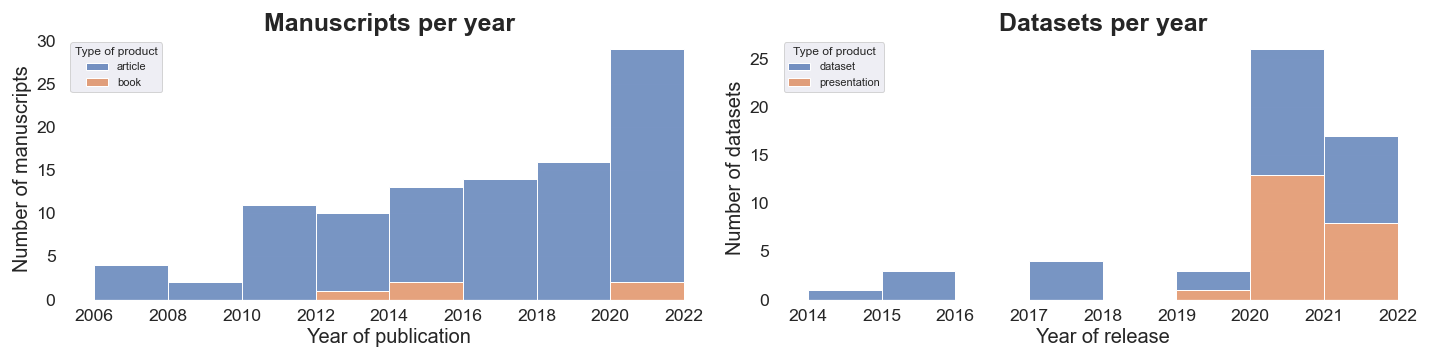
\includegraphics[width=\textwidth]{img/products_per_year.png}
\end{figure}

{\normalfont In the vast majority of papers published in peer-reviewed international journals, I am listed either as \textbf{first or last} (senior) author. Generally, my name is positioned prominently on the authors' list. Several of my papers were either \textbf{led or co-authored by students or postdoctoral researchers} whom I mentored.}

\begin{figure}[h]
\centering
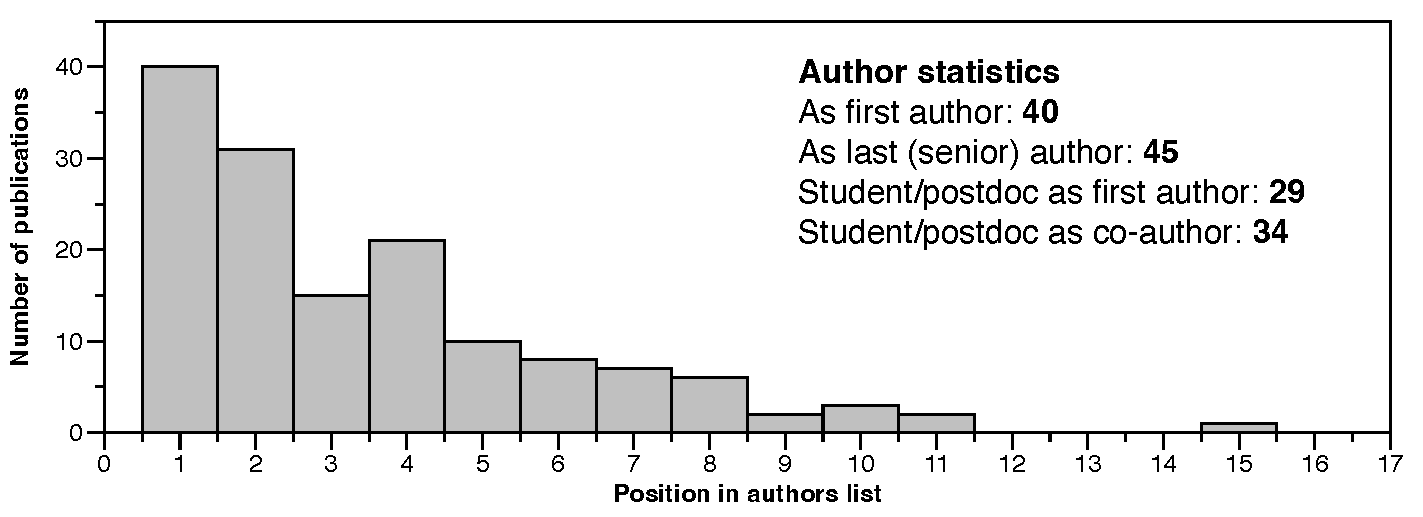
\includegraphics[width=0.8\textwidth]{img/Manuscripts.pdf}
\end{figure}

{\normalfont I have \textbf{107 documents} listed in Scopus, with \textbf{4,253 citations} and an \textbf{h-index of 38}. These metrics are slightly higher on Google Scholar, as it considers a broader range of research products. My metrics on Web of Science are distributed across several automatically generated profiles, which can affect the accuracy of citation counts and other metrics.}

\begin{figure}[h]
\centering
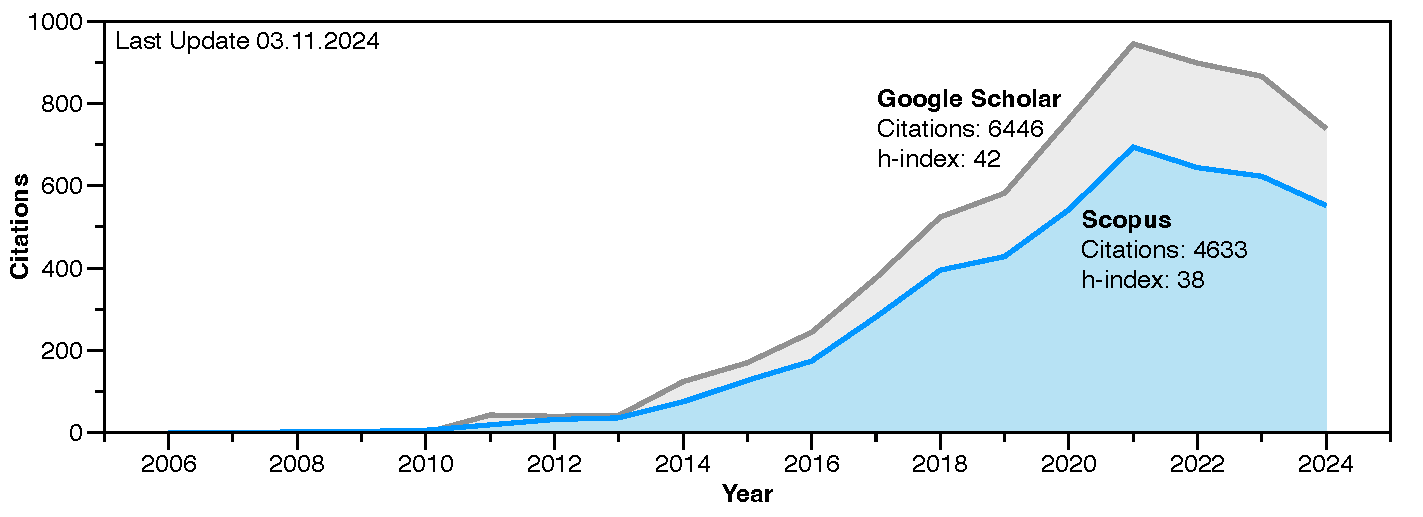
\includegraphics[width=0.8\textwidth]{img/CITATIONS.pdf}
\end{figure}

\newpage

{\normalfont Most of the papers I co-authored were published in journals classified as Q1 by the Journal Citation Reports 2022 (Web of Science). My scientific output encompasses a range of journals, from sector-specific publications with impact factors between 1 and 5 to high-impact journals with impact factors above 10 (Journal Citation Reports 2022 Impact Factor 2022)}

\begin{figure}[h]
\centering
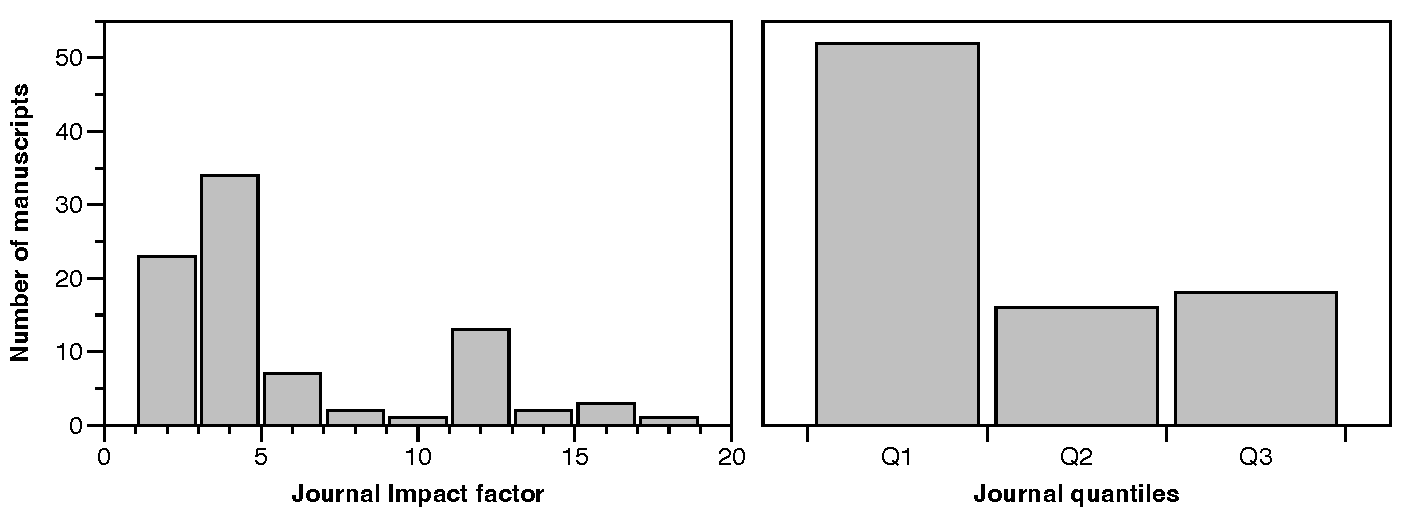
\includegraphics[width=0.8\textwidth]{img/Quantiles.pdf}
\end{figure}

{\normalfont The journals I publish in generally fall within the physical geography and geosciences category. Additionally, I have published papers in fields closely related to marine and coastal geomorphology, as well as remote sensing.}

\begin{figure}[h]
\centering
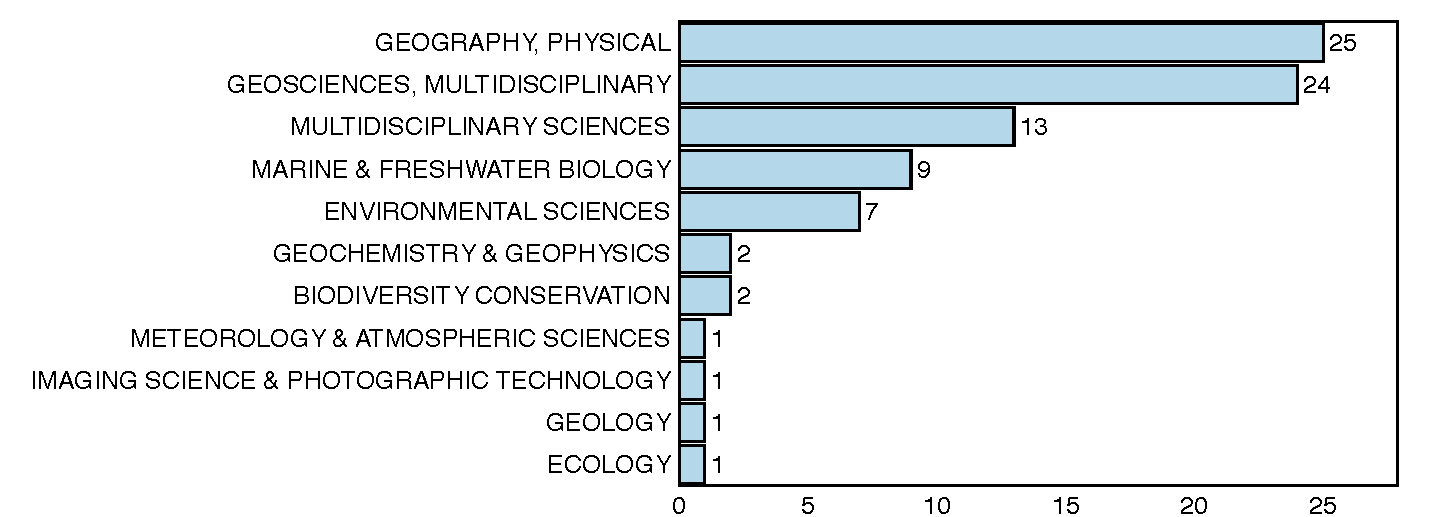
\includegraphics[width=0.8\textwidth]{img/topics.pdf}
\end{figure}

\section{10-years research impact (2013 - 2022)}
\bigskip

{\normalfont An overview of the impact of my research activities from 2013 to 2022 can be gathered from SciVal, a platform developed by Elsevier for analyzing bibliometric research output. According to SciVal, my research during this period includes 74 outputs, which have been cited 3,493 times. Below are some statistics extracted from SciVal (2013 - 2022).}
\smallskip

{\footnotesize 
\begin{description}
  \item [39.2\%] of my publications are in the top 10\% most cited publications worldwide.
  \item [66.7\%] of my publications are in the top 10\% journals by CiteScore.
  \item [Q1] 88.4\% of my publications are journals classified as Q1 by CiteScore. The others are in Q2 journals.
  \item [2.70] is my average Field-Weighted Citation Impact. Field-Weighted Citation Impact (FWCI) in SciVal indicates how the number of citations received my publications compares with the average number of citations received by all other similar publications. A FWCI of more than 1.00 indicates above the global average for similar publications. 2.70 means that my publications receive 170\% more citation than average.
\end{description}}

\newpage
\section{Media reports}
{\normalfont My research activities were reported by several media outlets, including newspapers, radios, TV channels, and websites I report the main media reports hereafter.}\\
{\footnotesize 
\begin{description}
  \item [2023] "Ancient warning of a rising sea" (Washington Post, Press, International)
  \item [2023] "Il livello del mare sta salendo. E le nostre coste sono a rischio" (Domani, Press, National) 
  \item [2023] "Ambiente, lo studio: "Livello mare nel 2100 fino a un metro in più rispetto a oggi" (Sky Tg 24, Web Press, National) 
   \item [2023] "Cambiamento climatico e gas serra, nel 2100 il livello del mare può aumentare di un metro: laguna di Venezia sorvegliata speciale" (Il Gazzettino, Web Press, National) 
  \item [2023] "Il nuovo report sul cambiamento climatico: Il mare invaderà certamente le coste, ma possiamo agire per rallentare il fenomeno" (La Stampa, Press, National) 
  \item [2023] "Aruba’s Bocas: home to the rarest fossil reefs on the planet!" (Aruba today, Web Press, International) 
  \item [2022] "Se sparisse il ghiaccio dei Poli..." (Focus, Press, National) 
  \item [2021] "Surprisingly fast ice-melts in past raise fears about sea level rise" (Horizon Magazine, Web Press, National) 
  \item [2021] "E se il mare del passato fosse stato più basso di quanto crediamo?" (Oggiscienza, Press, National) 
  \item [2020] "La sfida delle inondazioni, sempre più violente e frequenti" (Le Scienze, Press, National) 
  \item [2020] "South African seas up to 30m higher show a wet planet under siege" (Daily Maverick, Press, International) 
  \item [2020] "Sea-level rise projections can improve with state-of-the-art model" (Science Daily, Press, International) 
  \item [2017] "Ancient storms could have hurled huge boulders, scientists say" (Washington post, Press, International) 
  \item [2017] "Drohnen liefern detailreiche Einblicke in Korallenriffe" (Der Standard, Press, International) 
  \item [2017] "Mit Drohnen über dem Korallenriff" (Deutschland Radio, Radio, International) 
  \item [2017] "Riffe schützen Inseln vor Monsterwellen. Die Welle" (Die Welle, Web press, International) 
  \item [2017] "Drohnen für die Wissenschaft" (Arte TV, Television, International) 
  \item [2017] "Mit Drohnen gegen die Korallenbleiche" (Welt, Television, International) 
  \item [2016] "I droni contro l’erosione delle coste" (Dronezine, Press, National) 
  \item [2015] "Quatre chercheurs au milieu des surfeurs" (La Depeche de Tahiti, Press, International) 
  \item [2013] "Il business che spinge la startup é l’ecosistema costiero" (Il Secolo XIX, Press, National) 
  \item [2013] "How High Could the Tide Go?" (New York Times, Press, International) 
  \item [2011] "I protagonisti della ricerca scientifica in mare si raccontano" (SubAqua magazine, Press, National) 
\end{description}}

\section{Outreach}
{\normalfont I actively engage in sharing my scientific work through content creation on social media channels, with a keen interest in science communication. For instance, a recent video produced by Ca' Foscari featuring my expertise garnered approximately 67.000 views on TikTok and 29.000 on Instagram.}
\bigskip

\bigskip
\subsection{YouTube  $|$ {\normalfont\textit{@CoastalScience}}}
{\footnotesize I create and share videos on field techniques, geographic information systems, and daily fieldwork routines. I have 395 subscribers, and my videos have been streamed approximately 52.000 times, with a total watch time of nearly 3.000 hours.}
\bigskip

\subsection{Podcast  $|$ {\normalfont\textit{Storie di Mare}}}
{\footnotesize I produce a podcast called "Storie di Mare," where I use storytelling to educate listeners about coastal and marine processes. My episodes have been streamed approximately 2.400 times, and I share my podcasts on platforms like Spotify, YouTube, and Amazon Music.}
\bigskip

\subsection{Environmental education  $|$ {\normalfont\textit{Sons of the Ocean}}}
{\footnotesize I collaborate with "Sons of the Ocean," a non-profit organisation focused on environmental education for school-age children and youth. My contributions include providing media content, such as video commentaries on social media, and delivering presentations aimed at science outreach.}
\bigskip

\newpage

\begin{center}
    {\fontsize{36}{36}\selectfont\interthin Alessio \interheavy Rovere} \\ \bigskip
    {\fontsize{14}{14}\selectfont\interthin Publications list - Lista delle pubblicazioni}\\ \bigskip
        {\color{icnclr}} {Names of postdocs, Ph.D. students and master students \\ under my supervision while the article was published are \underline{underlined}}
\bigskip

        {\color{icnclr}} \textit{{I nomi di assegnist*, student* di dottorato e student* magistrali \\ che erano sotto la mia supervisione al momento della pubblicazione sono \underline{sottolineati}.}}



\end{center}

\nocite{*}
\section{Books and Book chapters}
\printbibliography[type=book,heading=none]

\section{Articles in international journals}
\printbibliography[type=article,heading=none]

\section{Other peer-reviewed articles}
\printbibliography[type=periodical,heading=none]

\section{Open-access datasets}
\printbibliography[type=dataset,heading=none]

\section{Selected presentations}
\printbibliography[type=misc,heading=none]


\end{document}